\documentclass[12pt,twoside]{report}


\usepackage[utf8]{inputenc}
\usepackage[a4paper,width=150mm,top=25mm,bottom=25mm,bindingoffset=6mm]{geometry}
\usepackage{graphicx}
\graphicspath{ {images/} }

\usepackage[backend=bibtex,style=alphabetic,sorting=none]{biblatex}
\addbibresource{tex/references.bib}

\usepackage{fancyhdr}
\pagestyle{fancy}
\rhead{}

\usepackage{float}

\usepackage{bm}
\usepackage{datetime}
\usepackage{hyperref}

\usepackage{algorithm}
\usepackage{algpseudocode}
\usepackage{amsmath}
\usepackage{amsfonts}
\usepackage{mathtools}

\usepackage{color}


%% Definitions %%

% ForEach loop
\algnewcommand\algorithmicforeach{\textbf{for each}}
\algdef{S}[FOR]{ForEach}[1]{\algorithmicforeach\ #1\ \algorithmicdo}

% Break
\newcommand{\Break}{\State \textbf{break} }

% Input
\algnewcommand\algorithmicinput{\textbf{Input:}}
\algnewcommand\Input{\item[\algorithmicinput]}

% Output
\algnewcommand\algorithmicoutput{\textbf{Output:}}
\algnewcommand\Output{\item[\algorithmicoutput]}

\newcommand{\R}{\mathbb{R}}  % Pretty set of real numbers.
\newcommand{\N}{\mathbb{N}}  % Pretty set of natural numbers.
\newcommand{\T}{\text{T}}  % Pretty transpose.
\newcommand{\mi}{\mathrm{i}}  % Pretty imaginary unit.
\DeclarePairedDelimiter{\ceil}{\lceil}{\rceil}  % The ceiling function.
\DeclarePairedDelimiter{\floor}{\lfloor}{\rfloor}  % The floor function.

\newcommand{\vect}[1]{\bm{\MakeLowercase{#1}}}  % Pretty vectors.
\newcommand{\mat}[1]{\mathbf{#1}}  % Pretty matrices.

\DeclareMathOperator*{\argmin}{argmin}  % Argmin
\DeclareMathOperator*{\argmax}{argmax}  % Argmax

% Inner product
\DeclarePairedDelimiterX{\inp}[2]{\langle}{\rangle}{#1, #2}


% Document collection
\newcommand{\doccount}{N}
\newcommand{\streamlen}{T}




%% Document %%


\begin{document}


% Title page
\begin{titlepage}
	\begin{center}
		\vspace*{1cm}
		
		\LARGE
		Bachelor thesis
		
		\Huge
		\textbf{Online Event Detection from Text Data}
		
		\vspace{1.5cm}
		
		\Large
		\textbf{Tomáš Kala}

		\vspace{1cm}

		\Large
		Supervisor: doc. Ing. Jiří Kléma, PhD.
		
		\vfill

		\includegraphics[width=0.4\textwidth]{lion}
		
		\Large
		Department of Computer Science\\
		Faculty of Electrical Engineering\\
		Czech Technical University in Prague\\
		\monthname, \the\year
	\end{center}
\end{titlepage}


% Abstract
\thispagestyle{plain}

\begin{center}
	\Large
	\textbf{Abstract}
\end{center}

Event detection is a process of analysis of text documents aiming to uncover real events happening in the world. It is based on the assumption that words appearing in similar documents and time windows are likely to concern the same real-world event. Therefore, our method attempts to group together words with similar temporal and semantic characteristics while discarding noisy words, not contributing to anything of interest. This results in a concise event representation through a set of representative keywords. These are then used to query the document collection to retrieve the actual event-related documents. Finally, we extract short summaries from these documents and annotate the events in a human-readable fashion. The keyword retrieval phase of our method is based on an existing event detection system, which we modify by employing a word embedding model to measure semantic similarity. The method is evaluated on a collection of 2 million documents from Czech news over a 13 months period and compared to the original method, not depending on word embeddings.
\\
\\
\textbf{Keywords:} Document retrieval, event detection, multi-document summarization, word embedding.

\hfill

\begin{center}
	\Large
	\textbf{Abstrakt}
\end{center}

Detekce událostí je proces analýzy textových dokumentů za účelem odhalení událostí, které se během doby jejich vydání staly ve světě. Tento proces je založen na předpokladu, že sémanticky podobná slova se zvýšeným výskytem během stejného období se pravděpodobně vztahují ke stejné události. Námi zkoumaná metoda se tedy snaží shlukovat dohromady slova s podobnou časovou nebo sémantickou charakteristikou, a zároveň ignorovat slova nenesoucí žádnou informaci. To vede k jednoduché reprezentaci událostí pomocí skupin klíčových slov. Tato klíčová slova jsou následně použita k dotazu do zkoumané kolekce a získání dokumentů vztahujících se k jednotlivým událostem. Z těchto dokumentů jsou nakonec extrahována krátká shrnutí pro bohatší popis událostí. Fáze získávání klíčových slov je založena na existujícím postupu, který modifikujeme použitím modelu vnořování slov (word embedding) k měření sémantické podobnosti. Metoda je vyhodnocena na kolekci 2 milionů dokumentů z českých novinových serverů vydané za období 13 měsíců, a porovnána s původním postupem nevyžadujícím vnořování slov.
\\
\\
\textbf{Klíčová slova:} Získávání dokumentů, detekce událostí, sumarizace více dokumentů, word embedding.


% Declaration
\chapter*{Declaration}
This is my declaration.


% Acknowledgements
\chapter*{Acknowledgements}
These are my acknowledgements.


% Table of contents
\tableofcontents
\listoffigures
\listofalgorithms


% Chapters
\chapter{Introduction}
%\addcontentsline{toc}{chapter}{Introduction}
As the number of news articles published each day grows, it becomes impossible to manually examine them all to learn about events happening in the world. The field of Event Detection arose as a subfield of Information Retrieval \citep{information-retrieval-2, information-retrieval} and Topic Detection and Tracking \citep{tdt, tdt-2} with a goal to aid the users by automatically discovering important events in document collections.

More precisely, given a stream of text documents published over a certain time period, the task is to analyze them and output a collection of events that happened in the world during the period. An event is loosely defined as \textit{something happening in a certain place at a certain time} \citep{retrospective-online-study}.

In this thesis, we chose to modify an approach introduced by \cite{event-detection}, which is a retrospective \footnote{Discussed in \autoref{sec:related-event-detection}} method relying on event representation through keywords. We build upon this method to incorporate a more advanced way of measuring semantic similarity between words, as well as propose an alternative algorithm for the event detection itself. Furthermore, we use the results to generate a more human-readable event representation than a simple set of keywords.

The rest of the thesis is organized as follows. First, in \autoref{chap:related-work}, we are going to discuss related work. Then, in \autoref{chap:data-preprocessing}, we describe the document collection used for evaluation and the preprocessing steps taken.

In \autoref{chap:word-analysis}, we describe the original paper's procedure used to extract temporal characteristics of the individual words. These characteristics are then examined to reveal a subset of words which may be related to certain events, as opposed to generally appearing noisy words, so called \textit{stopwords}. Then, we will proceed to the event detection itself.

In the original paper, the semantic similarity between two words is computed in only a simple manner in terms of their document overlap. We replace this coarse measure by applying the recent advances in word embeddings, hopefully obtaining a finer measure of word similarity. This will be more discussed in \autoref{chap:event-detection}.

Although a set of related keywords provides a concise event representation, it is not particularly readable to the user. In \autoref{chap:document-retrieval}, we follow by interpreting each keyword set as a query to the document collection. This allows us to employ information retrieval techniques to obtain documents relevant to each event.

Since the number of documents may be still too high, we also generate a short annotation for each event. The user can quickly skim through these annotations to get an idea what the events are about, and decide which of them are worth a closer examination. This will be addressed in \autoref{chap:event-annotation}.

Finally, we evaluate our method and compare it to the original paper in \autoref{chap:evaluation}. We then conclude the thesis in \autoref{chap:conclusion}.

\begin{figure}[H]
  \centering
  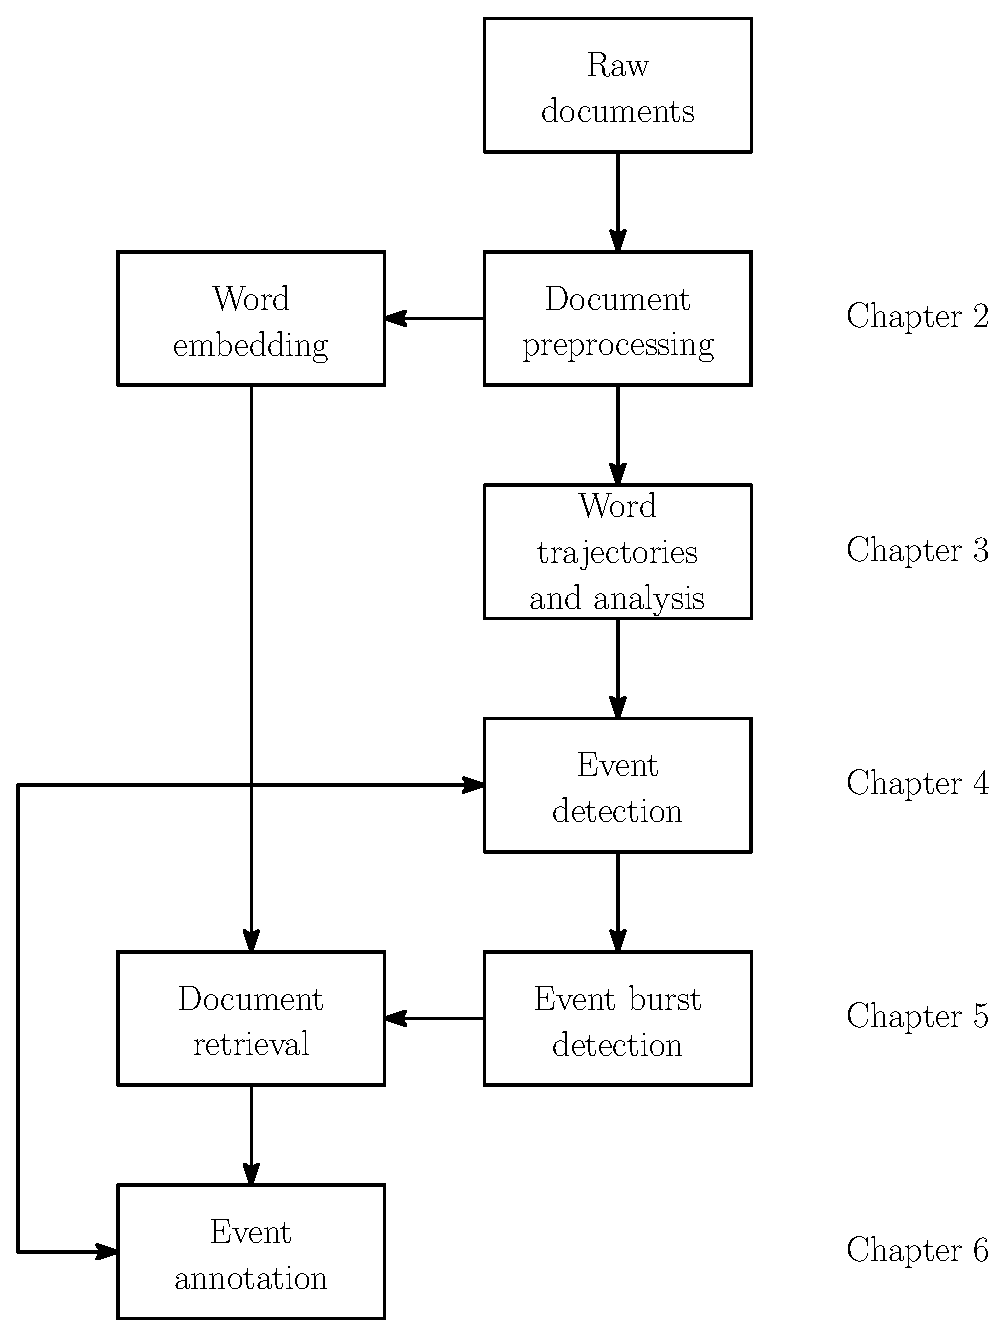
\includegraphics[height=0.6\paperheight]{diagram}
  \caption{Schematic representation of our method.}
  \label{fig:diagram}
\end{figure}

\chapter{Data preprocessing}
The collection we work with comes directly from webscraping without any special structure. The documents consist only of headlines, bodies and publication days. Furthermore, there are some noisy patterns such as residual HTML entities, typos, words cut in the middle, etc. To make the most of the following methods, we preprocess the documents to remove as many of these errors as possible, and also to gain some additional information about the text.

We will first employ some NLP methods to gain insight into the data. Then, we will train a model to obtain word embeddings.

Since most machine learning methods rely on the data being represented numerically, usually in a vector space, it is necessary to obtain such representation from the basic words we work with. Preferably, these vectors should retain as much information as possible. There are many ways to do so --- a simple TFIDF representation \cite{information-retrieval} which represents the words by weighted counts of their appearance in the document collection. More complicated methods, such as Latent Semantic Indexing \cite{lsi} attempt to discover latent structure within words to also reveal topical relations between them. This idea is further pursued by probabilistic topical models, such as Latent Dirichlet Allocation \cite{lda}.

In this thesis, we use the \textit{word2vec} model introduced by Tomáš Mikolov \cite{distributed-representations, linguistic-regularities, word2vec}, which uses a shallow neural network to project the words from some vocabulary into a vector space. Vectors in this space have interesting semantical properties, such as vector arithmetics preserving semantic relations, or semantically related words forming clusters.

Later on, we will need to measure word similarity. This will come up several times in the process of event detection --- in the event detection itself, later when querying the document collection to obtain documents related to the detected events, and finally to compute human-readable summaries. The word2vec models is fit for all of these uses, as opposed to the other mentioned approaches, some of which are designed only to measure document similarity, or, on the other hand, do not support document similarity queries very well.


\section{Document collection}
The input to the algorithm is a collection of $\doccount$ news documents containing full text articles along with their publication days, headlines and, possibly, additional metadata. We assume no preprocessing was done prior to running the algorithm.

If we denote $t_{i}$ as the publication day of a document $d_{i}$, the collection can be understood as a stream $\left\{ (d_{1}, t_{1}), (d_{2}, t_{2}), \dots, (d_{\doccount}, t_{\doccount}) \right\}$ with $t_{i} \leq t_{j}$ for $i < j$. Furthermore, we define $\streamlen$ to be the length of the stream (in days), and we normalize the document publication days to be relative to the document stream start; that is $t_{1} = 1$ and $t_{\doccount} = \streamlen$.


\section{Dataset}
{\color{red} TODO: Describe the dataset.}


\section{Preprocessing}
Some of the documents contain residual HTML entities from errors during web scraping, which we filter out using a manually constructed stopwords list.

We used the MorphoDiTa tagger \cite{morphodita} to perform tokenization, lemmatization and parts-of-speech tagging. Our whole analysis will be run on these lemmatized texts, and we will revert to the full forms only at the end when summarizing the events in a human-readable way.

{\color{red} TODO: Mikolov's phrase detection model?}


\section{Word embeddings} \label{word-embeddings}
Here, we will train the mentioned word2vec model. Although the training is time-consuming, the word vectors can be pre-trained on a large document collection and then reused in following runs, even on different documents.

For the training, we only discard punctuation marks and word denoted as unknown parts of speech my the tagger. Such unknown words are mostly typos or foreign language terms not important for our analysis. We do not remove any additional stopwords or parts of speech, as this would break word order, which is, to some extent, used by the word2vec model.

The thesis was implemented using the Gensim \cite{gensim} package. The project contains memory efficient, easy to use Python implementations of various topic modeling algorithms, word2vec included. In addition, we used the SciPy toolkit \cite{scipy} and Scikit-Learn \cite{scikit-learn} for various machine learning-related computations.

{\color{red} TODO: Describe the settings used in the algorithm (vector space dimensionality, avg/concat, etc.)}

\chapter{Event detection algorithm}
In this chapter, we describe the actual event detection algorithm. First, we describe the original method used by \cite{event-detection}. Then, we will make a change to incorporate semantic similarity through the word embeddings obtained in \autoref{chap:data-preprocessing}. Finally, we introduce an alternative algorithm that depends on word clustering using a custom distance function.

The original algorithm creates events as sets of related keywords by greedily minimizing a cost function combining temporal and semantical distance between words. However, the paper used only a simple notion of semantical distance, namely the document overlap between words. This demands that there exists at least one document containing all the words used to represent an event. This is a strong requirement, since the documents may use different vocabularies while conveying similar information.  As a result, the events are split into multiple keyword sets, leading to redundancy.

In an attempt to solve this problem, we modify the cost function, replacing the document overlap by Word2Vec-based similarity. This does not require the words to appear in exactly the same documents, only that they have similar semantics. We refer to this method as \textit{greedy approach}.

Realizing that the task of constructing keyword sets resembles the task of word clustering, we propose an alternative algorithm. Here, we apply a clustering algorithm to the words, using a modification of the cost function as a distance measure. This is a method referred to as \textit{cluster-based approach}.

First, we briefly describe the original method for referrence. This will make it clear which parts of the function we modify. It will also allow us to make reference to the original method in \autoref{chap:evaluation}, where we compare all three algorithms.

\section{Original method}
As stated in the introduction, the original method performs greedy minimization of a cost function defined over sets of words. The cost function consists of trajectory distance measuring the word distance in temporal domain, and document overlap, standing for distance in the semantic domain. We will first describe these two components and then combine them into the cost function.

\subsection{Trajectory distance}
Before measuring the trajectory distance, the trajectories are smoothened by fitting a probability density function to them. We adapt a similar technique in \autoref{chap:document-retrieval} where it is described in more detail. Our event detection modifications do not use it though, and we refer the reader to the original paper for more details.

After normalization to unit sum, the (smoothened) trajectory $\vect{\traj}_{w}$ of a word $w$ can be interpreted as a probability distribution over the stream days. The element $\traj_{w}(i)$ then denotes the probability that $w$ appears on day $i$. This interpretation allows to compare the trajectories using information-theoretic techniques, notably the information divergence.

In the original paper, the authors first defined the distance between trajectories of two words $v$ and $w$ as $\trajdist{\vect{\traj}_{v}}{\vect{\traj}_{w}} = \max \left\{ \kl{\vect{\traj}_{v}}{\vect{\traj}_{w}}, \kl{\vect{\traj}_{w}}{\vect{\traj}_{v}} \right\}$, symmetrizing the Kullback-Leibler divergence KL.

Then, the distance is generalized to a whole set of words $\featset$ as

\begin{equation}
	\text{Dist}( \featset ) = \max_{v, w \in \featset} \trajdist{\vect{\traj}_{v}}{\vect{\traj}_{w}}.
\end{equation}

\subsection{Document overlap}
The document overlap is again first defined for a pair of words $v$ and $w$ as $\text{DO}\left( v, w \right) = \frac{| \featset_{v} \cap \featset{w} |}{\min \left\{ | \featset_{v} |, | \featset_{w} | \right\}}$, where $\featset_{i}$ is the set of all documents containing the word $i$. The higher the document overlap, the more documents do the two words have in common, which them more likely to be correlated.

The overlap is again generalized to a set of words $\featset$ as

\begin{equation}
	\text{DO}( \featset ) = \min_{v, w \in \featset} \text{DO}( v, w ).
\end{equation}

\subsection{Cost function}
The cost function is a combination of the trajectory distance and document overlap of a set of words. It is defined as

\begin{equation}
	\text{C}( \featset ) = \frac{\text{Dist}( \featset )}{\text{DO}( \featset ) \cdot \sum_{w \in \featset} \text{DPS}_{w}}.
\end{equation}

Since the algorithm will attempt to minimize it, the intuitive result will be a set of words with with low trajectory distance and high document overlap. The algorithm will also prefer words of higher importance due to the last term of the denominator, counting in the power spectra.

\newpage

\subsection{Event detection algorithm}
The algorithm, called \textit{unsupervised greedy event detection algorithm} in the original paper, is defined as follows.

\begin{algorithm}[H]
\begin{algorithmic}[1]
\caption{Unsupervised greedy event detection}
\label{alg:greedy-event-detection}
\Input $\text{Word set} ~ \featset$

\State $\text{Sort the words in descending DPS order: } DPS_{w_{1}} \geq \dots \geq DPS_{w_{\left\vert \featset \right\vert}}$

\State $k = 0$

\ForEach{$w \in \featset$}
	\State $k = k + 1$	
	\State $e_{k} = \{ w \}$
	\State $cost_{e_{k}} = \frac{1}{DPS_{w}}$
	\State $\featset = \featset \setminus w$
	
	\While{$\featset \neq \emptyset$}
		\State $m = \argmin\limits_{m}{\text{C}( e_{k} \cup w_{m} )}$

		\If{$\text{C}( e_{k} \cup w_{m} ) < cost_{e_{k}}$}
			\State $cost_{e_{k}} = \text{C}( e_{k} \cup w_{m} )$
			\State $e_{k} = e_{k} \cup w_{m}$
			\State $\featset = \featset \setminus w_{m}$
		\Else
			\Break
		\EndIf
	\EndWhile
\EndFor

\Output $\text{Events} ~ \{ e_{1}, \dots, e_{k} \}$
\end{algorithmic}
\end{algorithm}


\begin{figure}[H]
  \centering
  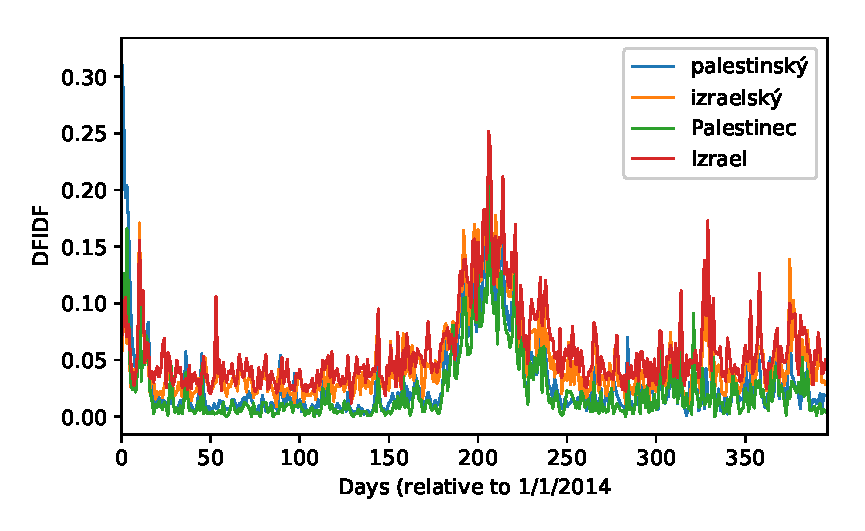
\includegraphics{original_event}  % original event
  \caption{Example of an event detected using the original method. The event consists of the words \textit{palestinian}, \textit{israeli}, \textit{Palestinian} and \textit{Israel}, respectively.}
  \label{fig:original-event}
\end{figure}


\section{Greedy approach}
Here, we describe the modifications done to the original method. We change the semantic similarity measure to take advantage of the Word2Vec model, and also redefine the trajectory distance accordingly, so it takes a similar form.

Both measures will be defined directly between a set of words $\featset$ and another word $w \notin \featset$.

\subsection{Trajectory distance}
We assume that the trajectories have been normalized to unit sum, as in the original method. The trajectory distance of $w$ to $\featset$ is again defined defined in terms of the Kullback-Leibler divergence as

\begin{equation}
	\trajdist{\featset}{w} = \kl{\vect{\bar{\traj}}_{\featset}}{\vect{\traj}_{w}},
\end{equation}

where $\vect{\bar{\traj}}_{\featset}$ is the mean of all trajectories of $\featset$ and $\vect{\traj}_{w}$ is the trajectory of $w$. The advantage is that, unlike in the original method, the divergences do not need to be precomputed between all pairs of words. The distance between a set and another word can be computed directly during the detection process, saving computation time.


\subsection{Semantic similarity}
Some of the astounding results of the Word2Vec model arise from semantically similar words forming clusters \citep{linguistic-regularities} in terms of cosine similarity, which is a standard measure used in information retrieval \citep{information-retrieval, cosine-similarity}.

The semantic similarity of $\featset$ and $w$ is defined in terms of cosine similarity as

\begin{equation}
	\semsim{\featset}{w} = \frac{\inp[\big]{\bar{\embed}_{\featset}}{\embed_{w}}}{\| \bar{\embed}_{\featset} \| \cdot \| \embed_{w} \|},
\end{equation}

where $\bar{\embed}_{\featset}$ is the mean of all vector embeddings of $\featset$ and $\embed_{w}$ is the vector embedding of $w$. Here, the mean vector represents the central topic of words in $\featset$.


\subsection{Cost function}
The cost function is defined similarly as in the original method:

\begin{equation} \label{eq:cost-function}
	\cost{\featset}{w} = \frac{\trajdist{\featset}{w}}{\exp(\semsim{\featset}{w}) \cdot \sum_{g \in \featset \cup w}{\text{DPS}_{g}}},
\end{equation}

Since the cosine similarity is bounded in $[-1, 1]$, we exponentiate it so that it is always positive. Otherwise, the cost function would reach negative values for highly dissimilar words, which would minimize it more than for similar ones.

Having constructed the cost function, we use Algorithm \ref{alg:greedy-event-detection} to detect events once again.


\begin{figure}[H]
  \centering
  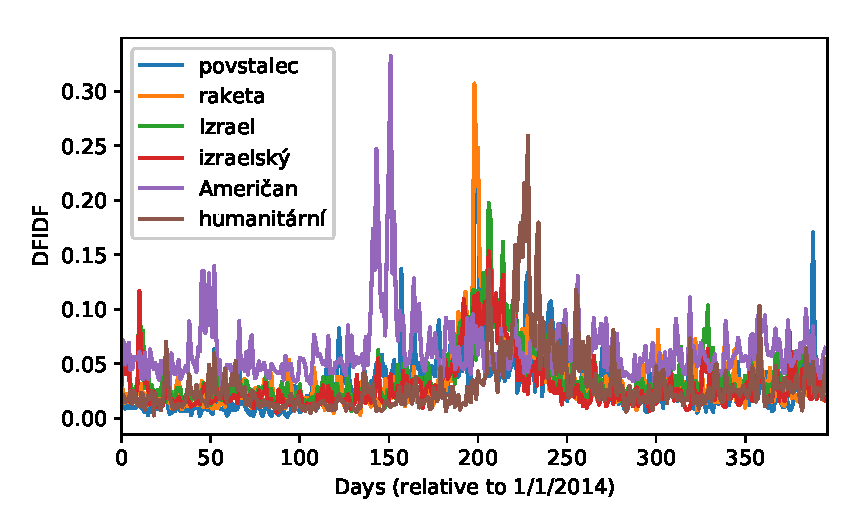
\includegraphics{greedy_event}  % greedy event
  \caption{Example of an event detected using the greedy method. The event consists of the words \textit{to shoot}, \textit{missile}, \textit{Israel} and \textit{israeli}, and is related to the same real event as \autoref{fig:original-event}.}
  \label{fig:greedy-event}
\end{figure}


\section{Cluster-based approach}
The final method interprets the task as literal clustering of words, using a custom distance function. The distance function will actually be a modification of the cost function yet again, though some means have to be taken to make it usable in this context. First, we need to consider a proper clustering algorithm.

The obvious requirement for the clustering algorithm is that it must not require an a priori knowledge of the desired number of clusters. Another requirement is that the algorithm must accept a custom distance measure.

We considered three candidate algorithms: Affinity propagation \citep{affinity-propagation}, DBSCAN \citep{dbscan} and its modification, HDBSCAN \citep{hdbscan}.

During our experimentation, Affinity propagation performed poorly, its clusters being often seemingly random and of low quality. The quality of HDBSCAN clusters was considerably better, though the algorithm took longer to converge as the number of eventful words grew. It also required to tune multiple parameters, which was difficult to do without any annotated data. We decided to use the DBSCAN algorithm, which outperformed Affinity propagation as well, and does not require to tune as many parameters as HDBSCAN.

In addition to the previously stated requirements, DBSCAN is also capable of filtering out noisy samples, not fit for any of the clusters. This property will prove advantageous for our task, as will become clear during the evaluation in \autoref{chap:evaluation}.


\subsection{Noise filtering}
Before we apply clustering, we will filter out the noisy parts from the word trajectories. Most words are on some level reported all the time, though only a fraction of these reportings corresponds to notable events. Unlike the greedy optimization described previously, clustering is prone to such noise, and would yield clusters of poor quality, often with trajectories being put together only due to their noisy parts being similar. With DBSCAN capable of filtering out noisy samples, quality words with some noise in their trajectories would be discarded.

We want to keep only those trajectory parts exceeding a certain frequency level, distinguishing notable bursts from the general noise. We do this by computing a cutoff value for each event trajectory and discarding the sectors falling under this cutoff. This procedure is adopted from \cite{online-search-queries}. The algorithm is based on computing a moving average along the trajectory, and works as follows:

\begin{algorithm}[H]
\begin{algorithmic}[1]
\caption{Burst filtering}
\label{alg:burst-filtering}
\Input $\text{window-length} \ l,\ \text{word trajectory} \ \vect{\traj_{w}}$

\State $\vect{MA}_{l} = \text{Moving Average of length} ~ l ~ \text{for} ~ \vect{\traj}_{w} = \left[ \traj_{w}(1), \traj_{w}(2), \dots, \traj_{w}(\streamlen) \right]$

\State $\mathit{cutoff} = \text{mean} \left( \vect{MA}_{l} \right) + \text{std} \left( \vect{MA}_{l} \right)$

\State $\vect{bursts}_{w} = \left[ \traj_{w}(t) \mid \traj_{w	}(t) > \mathit{cutoff} \right]$

\Output $\vect{bursts}_{w}$
\end{algorithmic}
\end{algorithm}


\subsection{Distance function}
We now define the distance function used by DBSCAN. It conveys similar information as the cost function in the previous two algorithms. We still need to measure the trajectory distance as well as semantic similarity between two words.

For a measure of trajectory distance, we replace the Kullback-Leibler divergence by the Jensen-Shannon divergence JSD, which is symmetric in its arguments. This is a necessary property of the distance function.

Instead of semantic \textit{similarity}, we measure semantic \textit{distance} as the Euclidean distance between two word vector embeddings. The reason is that Euclidean distance is unbounded, which makes it possible for the samples to be spread farther apart. Since DBSCAN is a density-based clustering algorithm, having high density areas consisting of words with low trajectory distance and similar cosine similarities would cause them to appear in the same cluster. This would cluster the words only in terms of their trajectories, not semantics.

The distance between two words $v$ and $w$ with trajectories $\vect{\traj}_{v},\ \vect{\traj}_{w}$ and embeddings $\embed_{v},\ \embed_{w}$ is now defined as

\begin{equation}
	\distfunc{v}{w} = \jsd{\vect{\traj}_{v}}{\vect{\traj}_{w}} \cdot \| \embed_{v} - \embed_{w}\|_{2},
\end{equation}

with $\jsd{\vect{p}}{\vect{q}} = \frac{1}{2} \left( \kl{\vect{p}}{\vect{m}} + \kl{\vect{q}}{\vect{m}} \right) ,\ \vect{m} = \frac{1}{2} \left( \vect{p} + \vect{q} \right)$.


\subsection{Event detection}
The input and output of the event detection algorithm remains the same as in Algorithm \ref{alg:greedy-event-detection}, only the internals are different. This makes it easy to swap the two algorithms for comparison.

\begin{algorithm}[H]
\begin{algorithmic}[1]
\caption{Cluster-based event detection}
\Input $\text{Word set} ~ \featset$

\State Precompute a distance matrix $\distmat \in \R^{\left\vert \featset \right\vert \times \left\vert \featset \right\vert}$ with $\distmat_{ij} = \distfunc{w_{i}}{w_{j}}$

\State Apply HDBSCAN to $\distmat$, obtaining $k$ clusters and the noisy cluster

\ForEach{$(w, cluster) \in \text{HDBSCAN.clusters}$}
	\If{$cluster \neq noise$}
		\State $e_{cluster} = e_{cluster} \cup w$
	\EndIf
\EndFor

\Output $\text{Events} ~ \{ e_{1}, e_{2}, \dots, e_{k} \}$
\end{algorithmic}
\end{algorithm}


\begin{figure}[H]
  \centering
  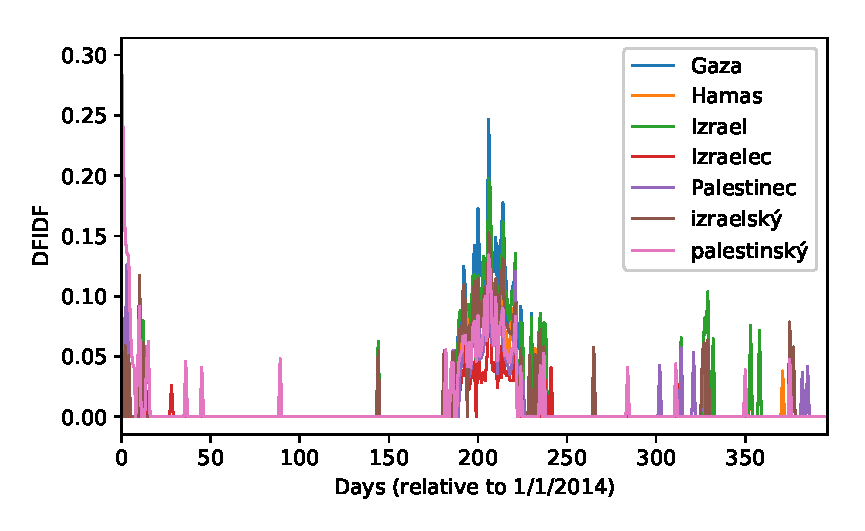
\includegraphics{cluster_event}  % cluster event
  \caption{Example of an event detected using the cluster-based method. The event is related to the same real event as \autoref{fig:original-event} and \autoref{fig:greedy-event}. Note that the trajectories are clear of noise due to application of Algorithm \ref{alg:burst-filtering}}
  \label{fig:cluster-event}
\end{figure}


\chapter{Event examination}
\section{Trajectory preprocessing}
During the event detection itself, we will need to measure the similarity of two trajectories. However, due to the general noisiness of the data, the similarities are not computed directly. Most features would then seem distant due to mild bursts malforming the trajectories, while not really contributing to the underlying events. Thus, the trajectories are first preprocessed.

\subsection{Burst filtering}
As we are only interested in the dominant bursts around the main events, we filter out the mild ones. We do this by computing a cutoff value for each feature trajectory and discarding all trajectory elements falling under this cutoff. This procedure is adopted from \cite{online-search-queries}. The algorithm is as follows:

\begin{algorithm}[H]
\begin{algorithmic}[1]
\caption{Burst filtering}
\Input $\text{window-length} ~ w$

\ForEach {$\vect{\traj}_{f} \in \{ \vect{\traj}_{1}, \vect{\traj}_{2}, \dots, \vect{\traj}_{\featcount}\}$}
	\State $\vect{MA}_{w} = \text{Moving Average of length} ~ w ~ \text{for} ~ \vect{\traj}_{f} = \left[ \traj_{f}(1), \traj_{f}(2), \dots, \traj_{f}(\streamlen) \right]$

	\State $\mathit{cutoff} = \text{mean} \left( \vect{MA}_{w} \right) + \text{std} \left( \vect{MA}_{w} \right)$

	\State $\vect{bursts}_{f} = \left[ \traj_{f}(t) \mid \traj_{f}(t) > \mathit{cutoff}, \traj_{f}(t) \in \vect{y}_{f} \right]$
\EndFor

\Output $\{ \vect{bursts}_{1}, \vect{bursts}_{2}, \dots, \vect{bursts}_{\featcount} \}$
\end{algorithmic}
\end{algorithm}

{\color{red} TODO: In the paper, they use $\vect{MA}(t)_{w} > \mathit{cutoff}$, try that. Also, why did I miss that? :(}

\subsection{Normalization}
From now on, we assume the individual trajectories have been normalized to have unit sums. This can be computed efficiently by vectorizing the operation and dividing every row of $\trajmat$ by its sum. Thanks to this normalization, the individual trajectories can be interpreted as probability distributions over the stream days.

\subsection{Smoothing}

We smoothen each trajectory by fitting a probability density function to it. Preserving the probability interpretation allows us to measure trajectory distance using information divergence later. Different techniques must be employed when smoothing aperiodic and periodic feature trajectories, since we aim mainly to fit all non-trivial bursts.

In this section, we interpret the trajectories as two-dimensional observations $\traj_{f} = \{ \left( 1, \traj \left(1 \right) \right), \left( 2, \traj \left(2 \right) \right), \dots, \left( \streamlen, \traj \left(\streamlen \right) \right) \}$.

\begin{enumerate}

\item \textbf{Aperiodic features}

An aperiodic feature trajectory $\traj_{f}$ is modeled by a Gaussian distribution. We fit the Gaussian function

\begin{equation*}
	f(x) = \frac{1}{\sigma \sqrt{2 \pi}} \exp(-\frac{\left( x - \mu \right)^{2}}{2 \sigma^{2}})
\end{equation*}

to the trajectory $y_{f}$. The parameters $\mu$ and $\sigma$ are estimated using non-linear Least squares method. Unlike \cite{event-detection} who use the EM algorithm, Least squares proved to be less prone to outliers, yielding a shape more resembling the actual trajectory.

\item \textbf{Periodic features}

A periodic feature trajectory $\traj_{f}$ is modeled using a mixture of $K = \floor{\streamlen / \text{DP}_{f}}$ Cauchy distributions as in \cite{health-events}:

\begin{equation*}
	f(x) = \sum_{k = 1}^{K}{\alpha_{k} \frac{1}{\pi} \left( \frac{\gamma_{k}}{\left( x - \mu_{k} \right)^{2} + \gamma_{k}^{2}} \right)}
\end{equation*}

The mixing parameters $\alpha_{k},\ \sum_{k = 1}^{K}{\alpha_{k}} = 1$, location parameters $\mu_{k}$ and scale parameters $\gamma_{k}$ are estimated using the EM algorithm.

The Cauchy distribution has a narrower peak and thicker tails than the Gaussian distribution, which models the periodic bursts more closely. The individual bursts of a periodic feature tend to be quite short, but even between two consecutive bursts, the frequency remains at a non-negligible level, which makes the Cauchy distribution a somewhat better choice.

\end{enumerate}

\chapter{Conclusion}
%\addcontentsline{toc}{chapter}{Conclusion}
We examined how event detection methods depending on keyword representation could be improved by considering word embedding models, namely the Word2Vec model \citep{word2vec}. We tried to augment an existing method by \cite{event-detection} to use a Word2Vec-based similarity function to match semantically related words together. This did not bring significant improvement -- although the detected events were richer and less redundant, a notable amount of noise appeared. This made the events hard to assign to their real world counterparts, as most of their keywords did not contribute to any underlying topic.

Then, we explored a different approach, where we interpreted the keyword-based event detection as a literal clustering task. We defined a custom distance function also utilizing the Word2Vec model as a semantic measure. We then applied a clustering algorithm equipped with this distance function to words previously selected as eventful. Our evaluation suggests that this method was more successful than both the original method and its Word2Vec modification. The resulting events were composed mostly of representative words and reached lesser redundancy and noisiness than the previous methods.

The disadvantage of both our methods is the necessity to train the Word2Vec model, which is time consuming. However, it can be trained once and than reused for subsequent detections, as long as the document vocabulary remains similar.

We also examined how the Word2Vec model could be used to retrieve documents concerning the detected events. We applied the Word Mover's Distance \citep{wmd} to documents within each event's bursty period as a measure of their relevance to that particular event's keyword set. We then selected the most relevant documents as the event's document representation. Although the documents were of high quality and represented the events well, the process took an unbearable amount of time. In the original method, the retrieval process was more straightforward and much more efficient.

Finally, we applied multi-document summarization techniques to the documents to obtain a short summary describing each event. This, along with the event's occurrence dates and document sets, are the outputs of our method presented to the user. The summaries serve the purpose of giving a quick reference of the event's topic, based on which the user may decide to examine the event further and go through the retrieved documents.

In future work, it would be beneficial to use a more efficient way of computing the documents relevant to each event. Traditional information retrieval techniques, such as Latent Semantic Indexing \citep{lsi} could be used here, perhaps with some domain specific knowledge of the underlying events, such as their bursty periods.

Also, we would like to examine how an event could be represented directly as a set of documents, rather than words. Although there are attempts to do so \citep{document-bursty-representation}, they require to fine-tune a number of parameters, and the document representation is again constructed using word trajectories. The Doc2Vec model \citep{doc2vec}, a generalization of Word2Vec able to embed whole documents in a vector space, could be used to obtain the semantic representation.

Instead of computing a cutoff value to clean a word or an event trajectory, as we did in \autoref{chap:event-detection}, further signal processing techniques could be applied on the trajectories to separate the dominant bursts from the underlying noise. The result would be a somewhat cleaner trajectory devoid of any milder bursts of no interest. This could lower the noisiness, since words would be matched together based on only the dominant activity, not any underlying influence, which still eludes the cutoff value method.


% Appendices
\appendix
\chapter{Appendix Title}
\input{tex/chapters/appendix}


% Bibliography
\printbibliography

\end{document}